\section{Results}\label{sec:results}

The main quantitave data can be seen in tables \ref{table:1} and \ref{table:2}.
These present a number of metrics for each model that was trained.
These are the number of true positives, false positives, false negatives, and true negatives, as well as accuracy (as computed in the SigNet paper\cite{sig_net}).
Additionally, the number of false positives and true negatives and the accuracy are computed and included after the forged image in each of the negative datapoints is perturbed as described is section \ref{my_fgsm}.
These metrics are shown for the 3 models (SigNet64, SigNet128, and SigNet256) which have dimensionality 64, 128, and 256 of their outputs (latent vectors).
All metrics are computed on the validation set.

\begin{table*}[t]
    \centering
    \begin{tabular}{|c | c >{\em}c | >{\em}c c | >{\bfseries}c | >{\em}c c >{\bfseries}c|}
    % \begin{tabular}{|m{2.5cm} | m{1cm} | m{1cm} | m{1cm} | m{1cm} | m{1cm} | m{1cm} | m{1cm} | m{1cm}|}
        \hline
        % lvd & tp & fn & fp & tn & acc & fpi & tni & acci\\ [0.1ex]
        % Dimensionality & true positive & false negative & false positive & true negative & accuracy & false positive imp & true negative imp & accuracy imp\\ [0.1ex]
        \multirow{3}{*}{Dimensionality} & \multicolumn{5}{c|}{Normal} & \multicolumn{3}{c|}{Adversarial}\\
        \hline
        & \multicolumn{2}{c|}{Positive} & \multicolumn{2}{c|}{Negative} & \multirow{2}{*}{Accuracy} & Positive & Negative & \multirow{2}{*}{Accuracy}\\
        % \hline
        & True & False & False & True & & False & True & \\
        \hline
        64 & 1144 & 4 & 236 & 1376 & 91.30 & 450 & 930 & 75.14\\
        128 & 1044 & 224 & 336 & 1156 & 79.71 & 1211 & 169 & 43.95\\
        256 & 729 & 88 & 651 & 1292 & 73.22 & 377 & 1003 & 62.75\\ [0.1ex]
        \hline
    \end{tabular}
    \caption{Comparison of Accuracy using Latent Vector Sizes after 5 Epochs}
    \label{table:1}
\end{table*}

\begin{table*}[t]
    \centering
    \begin{tabular}{|c | c >{\em}c | >{\em}c c | >{\bfseries}c | >{\em}c c >{\bfseries}c|}
    % \begin{tabular}{|m{2.5cm} | m{1cm} | m{1cm} | m{1cm} | m{1cm} | m{1cm} | m{1cm} | m{1cm} | m{1cm}|}
        \hline
        % lvd & tp & fn & fp & tn & acc & fpi & tni & acci\\ [0.1ex]
        % Dimensionality & true positive & false negative & false positive & true negative & accuracy & false positive imp & true negative imp & accuracy imp\\ [0.1ex]
        \multirow{3}{*}{Dimensionality} & \multicolumn{5}{c|}{Normal} & \multicolumn{3}{c|}{Adversarial}\\
        \hline
        & \multicolumn{2}{c|}{Positive} & \multicolumn{2}{c|}{Negative} & \multirow{2}{*}{Accuracy} & Positive & Negative & \multirow{2}{*}{Accuracy}\\
        % \hline
        & True & False & False & True & & False & True & \\
        \hline
        64 & 1347 & 0 & 33 & 1380 & 98.80 & 39 & 1341 & 97.39\\
        128 & 1366 & 0 & 14 & 1380 & 99.49 & 91 & 1289 & 96.20\\
        256 & 1353 & 0 & 27 & 1380 & 99.02 & 89 & 1291 & 95.80\\ [0.1ex]
        \hline
    \end{tabular}
    \caption{Comparison of Accuracy using Latent Vector Sizes after 20 epochs}
    \label{table:2}
\end{table*}

As mentioned in section \ref{sec:cedar_flaw}, there is at least one significant difference between the genuine and forge images in the CEDAR dataset.
Since CNNs are very powerful and should be able to pick up on this difference very easily, the CEDAR dataset is not a good test of an architecture's ability to understand or verfiy handwritten signatures.

\begin{figure}[h]
    \begin{center}
        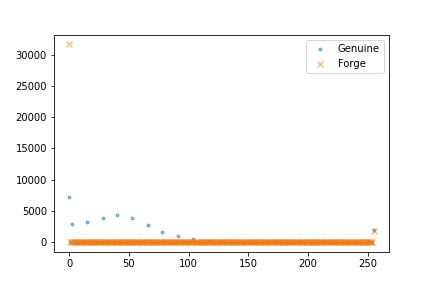
\includegraphics[width=0.8\linewidth]{mean_hist.png}
    \end{center}
    \caption{Histogram of Means of Binned Pixel Values}
    \label{fig:hist_pixel_values}
\end{figure}

% If I need more content, I could graph the training loss and talk about how it stabilzes.

% the accuracy after \_ amount of training was 72% accuracy
% It would take too long to get 100% accuracy

% The validation loss was higher than the training loss even on the 1st epoch of training.
% I believe this is because the images in the datapoints (image pairs with labels) have been seen before...


% random noise can score well...
